\chapter{Test Environment Setup and Verification}
\lhead{\emph{Appendix A - Test Environment Setup and Verification}}  

A dedicated environment has been developed for purposes of development testing. The environment comprises a Kubernetes cluster running a microservices-based pipeline application, supported by Kafka and Zookeeper instances. The pipeline application and messaging infrastructure run in dedicated Kubernetes namespaces  \textit{testbed} and  \textit{kafka}, respectively. Environment prerequisites, configuration and validation are detailed in the following sections.

\section{Prerequisites}
\begin{enumerate}
	
 \item Install a recent Java Development Kit on your host environment. 
	
 \item Install a recent Python runtime on your host environment. Additionally, install Kafka tools for Python:
 
 \begin{lstlisting}[language=bash]
 $ pip install kafka-python
 \end{lstlisting}

\item Install a recent version of Maven by following the instructions provided at:

https://maven.apache.org/users/index.html. 
	
 \item Install Docker by following the instructions appropriate for your OS. Documentation is available at https://docs.docker.com/install.
	
	
 \item Install Minikube by following the steps detailed at \linebreak https://kubernetes.io/docs/tasks/tools/install-minikube.

\end{enumerate}

\section{Configuration}

\begin{enumerate}
	
 \item The various required configuration scripts are bundled with the project implementation sources at https://github.com/schmigware/monitoring-app. Clone this repository to your local environment by issuing following command: 

\begin{lstlisting}[language=bash]
$ git clone https://github.com/schmigware/monitoring-app
\end{lstlisting}

 \item Start the Minikube Kubernetes cluster by executing the script \texttt{config/startcluster.sh}

\begin{lstlisting}[language=bash]
$ cd kubernetes
$ ./startcluster.sh
\end{lstlisting}

Minikube will echo startup status to the console.

\begin{figure}[H]
	\centering  
	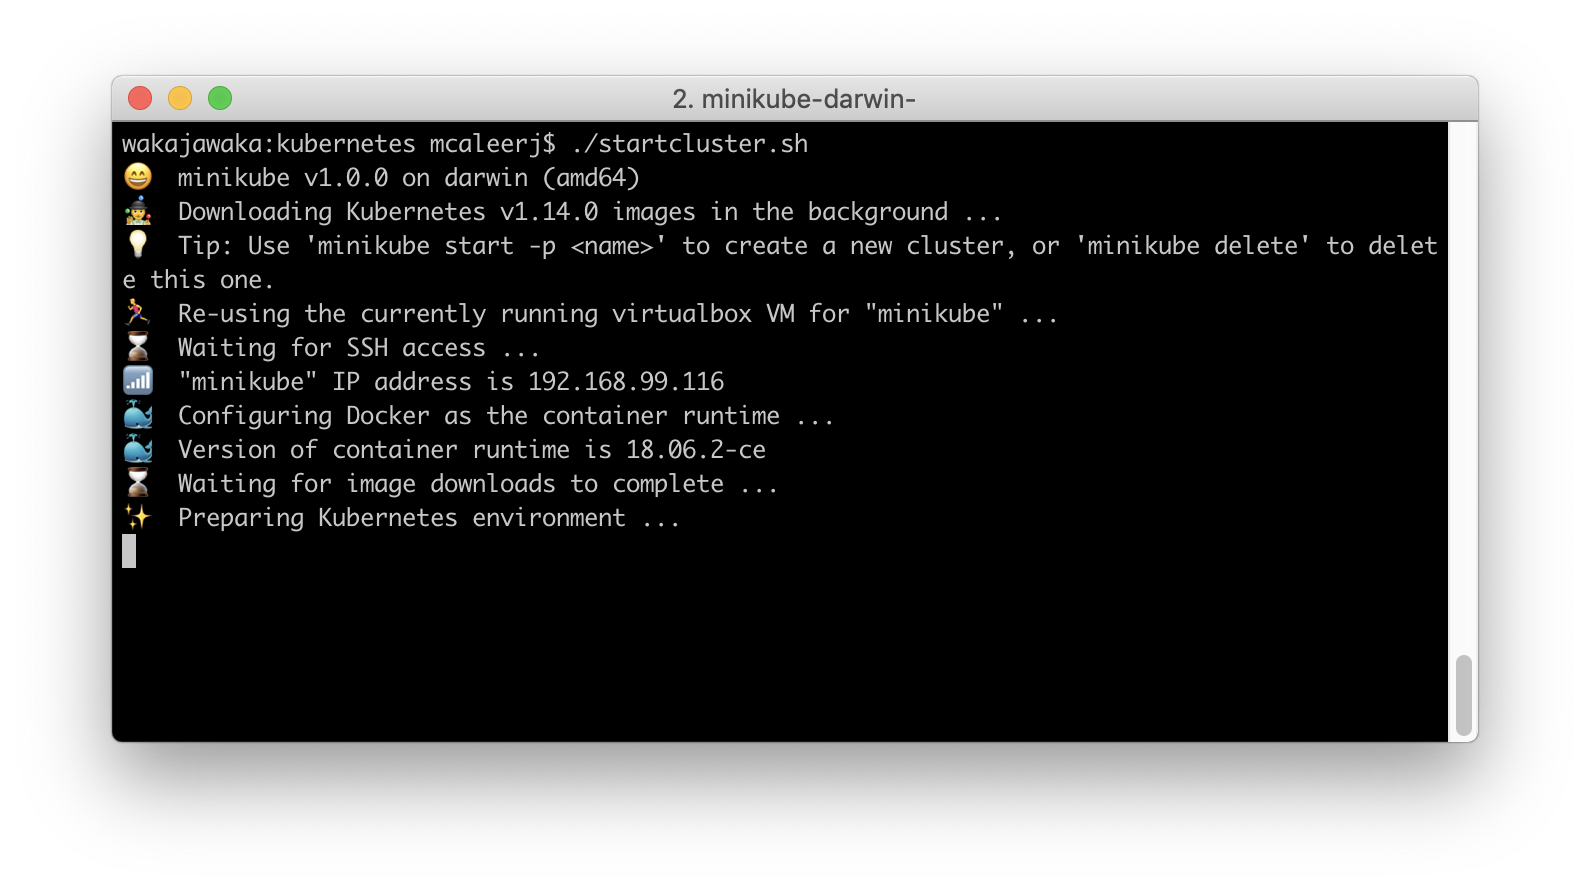
\includegraphics[width=\linewidth]{figures/appendixA/minikube-startup.png}
	\caption{Minikube cluster startup.}
\end{figure}


 \item The Zookeeper/Kafka configuration files bundled with the project are customised versions of those provided by open source project https://github.com/Yolean/kubernetes-kafka. A single Kafka broker is defined; importantly, auto-creation of Kafka topics is enabled for the cluster. To create the various required namespaces and services, execute the script \texttt{config/configurecluster.sh}. Cluster configuration may take several minutes while persistent volumes are initialised.

\begin{lstlisting}[language=bash]
$ ./configurecluster.sh
\end{lstlisting}


 \item Verify that the \texttt{kafka} namespace has been created correctly by issuing the following kubctl command:
 
 \begin{lstlisting}[language=bash]
 $ kubectl get namespaces
 \end{lstlisting}

The output should list the expected namespace.

\begin{figure}[H]
	\centering  
	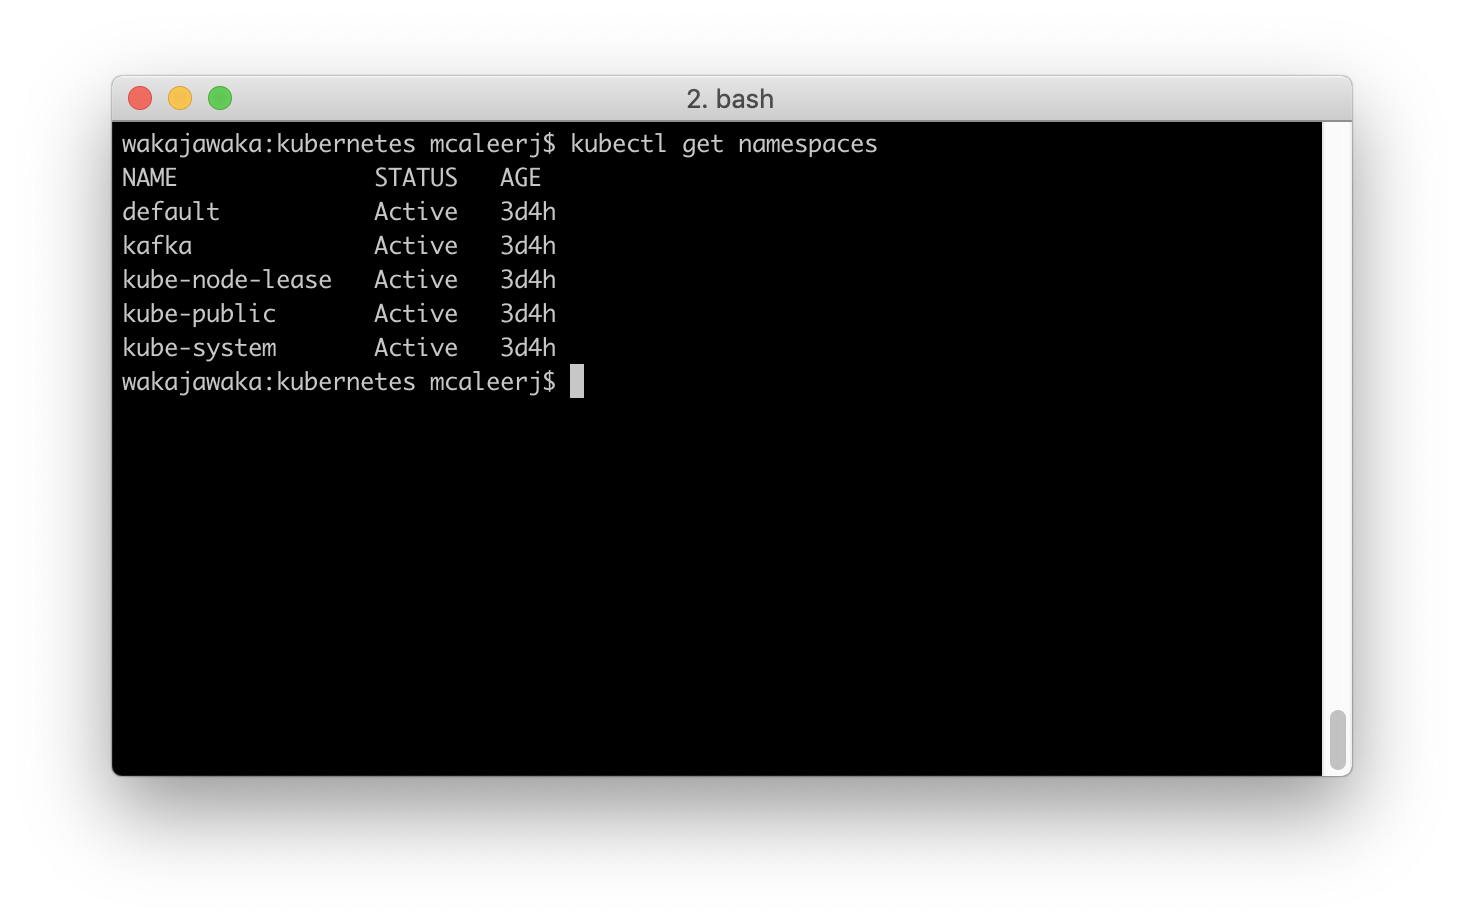
\includegraphics[width=\linewidth]{figures/appendixA/namespaces.png}
	\caption{Verification of kafka namespace creation.}
\end{figure}

 \item Verify that the \texttt{kafka} namespace contains running Kafka and Zookeeper pods by issuing the following kubctl command, which lists all pods for the namespace in question:

\begin{lstlisting}[language=bash]
$ kubectl get pods -n kafka
\end{lstlisting}

The output should contain Kafka and Zookeeper pods.

\begin{figure}[H]
	\centering  
	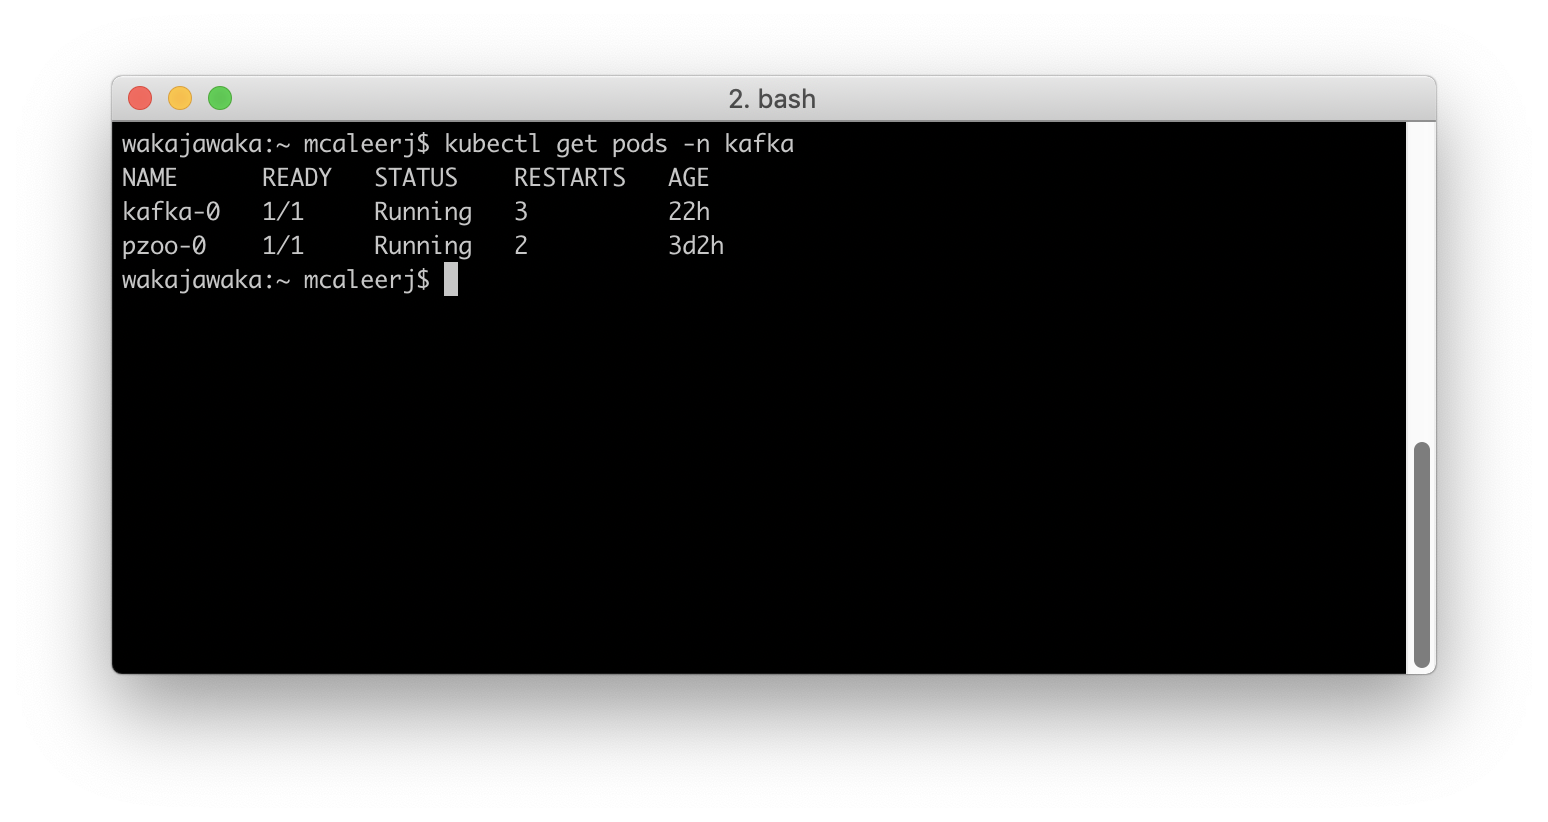
\includegraphics[width=\linewidth]{figures/appendixA/kafka-pods.png}
	\caption{Verification of Zookeeper/Kafka pod creation.}
\end{figure}


 \item Cluster state can be further verified via the Minikube Dashboard. To start the dashboard, issue the following command:
 
 \begin{lstlisting}[language=bash]
 $ minikube dashboard
 \end{lstlisting}
 
 When the dashboard opens, navigate to the \texttt{kafka} namespace. Workload status images should be displayed in green. 
 
 \begin{figure}[H]
 	\centering  
 	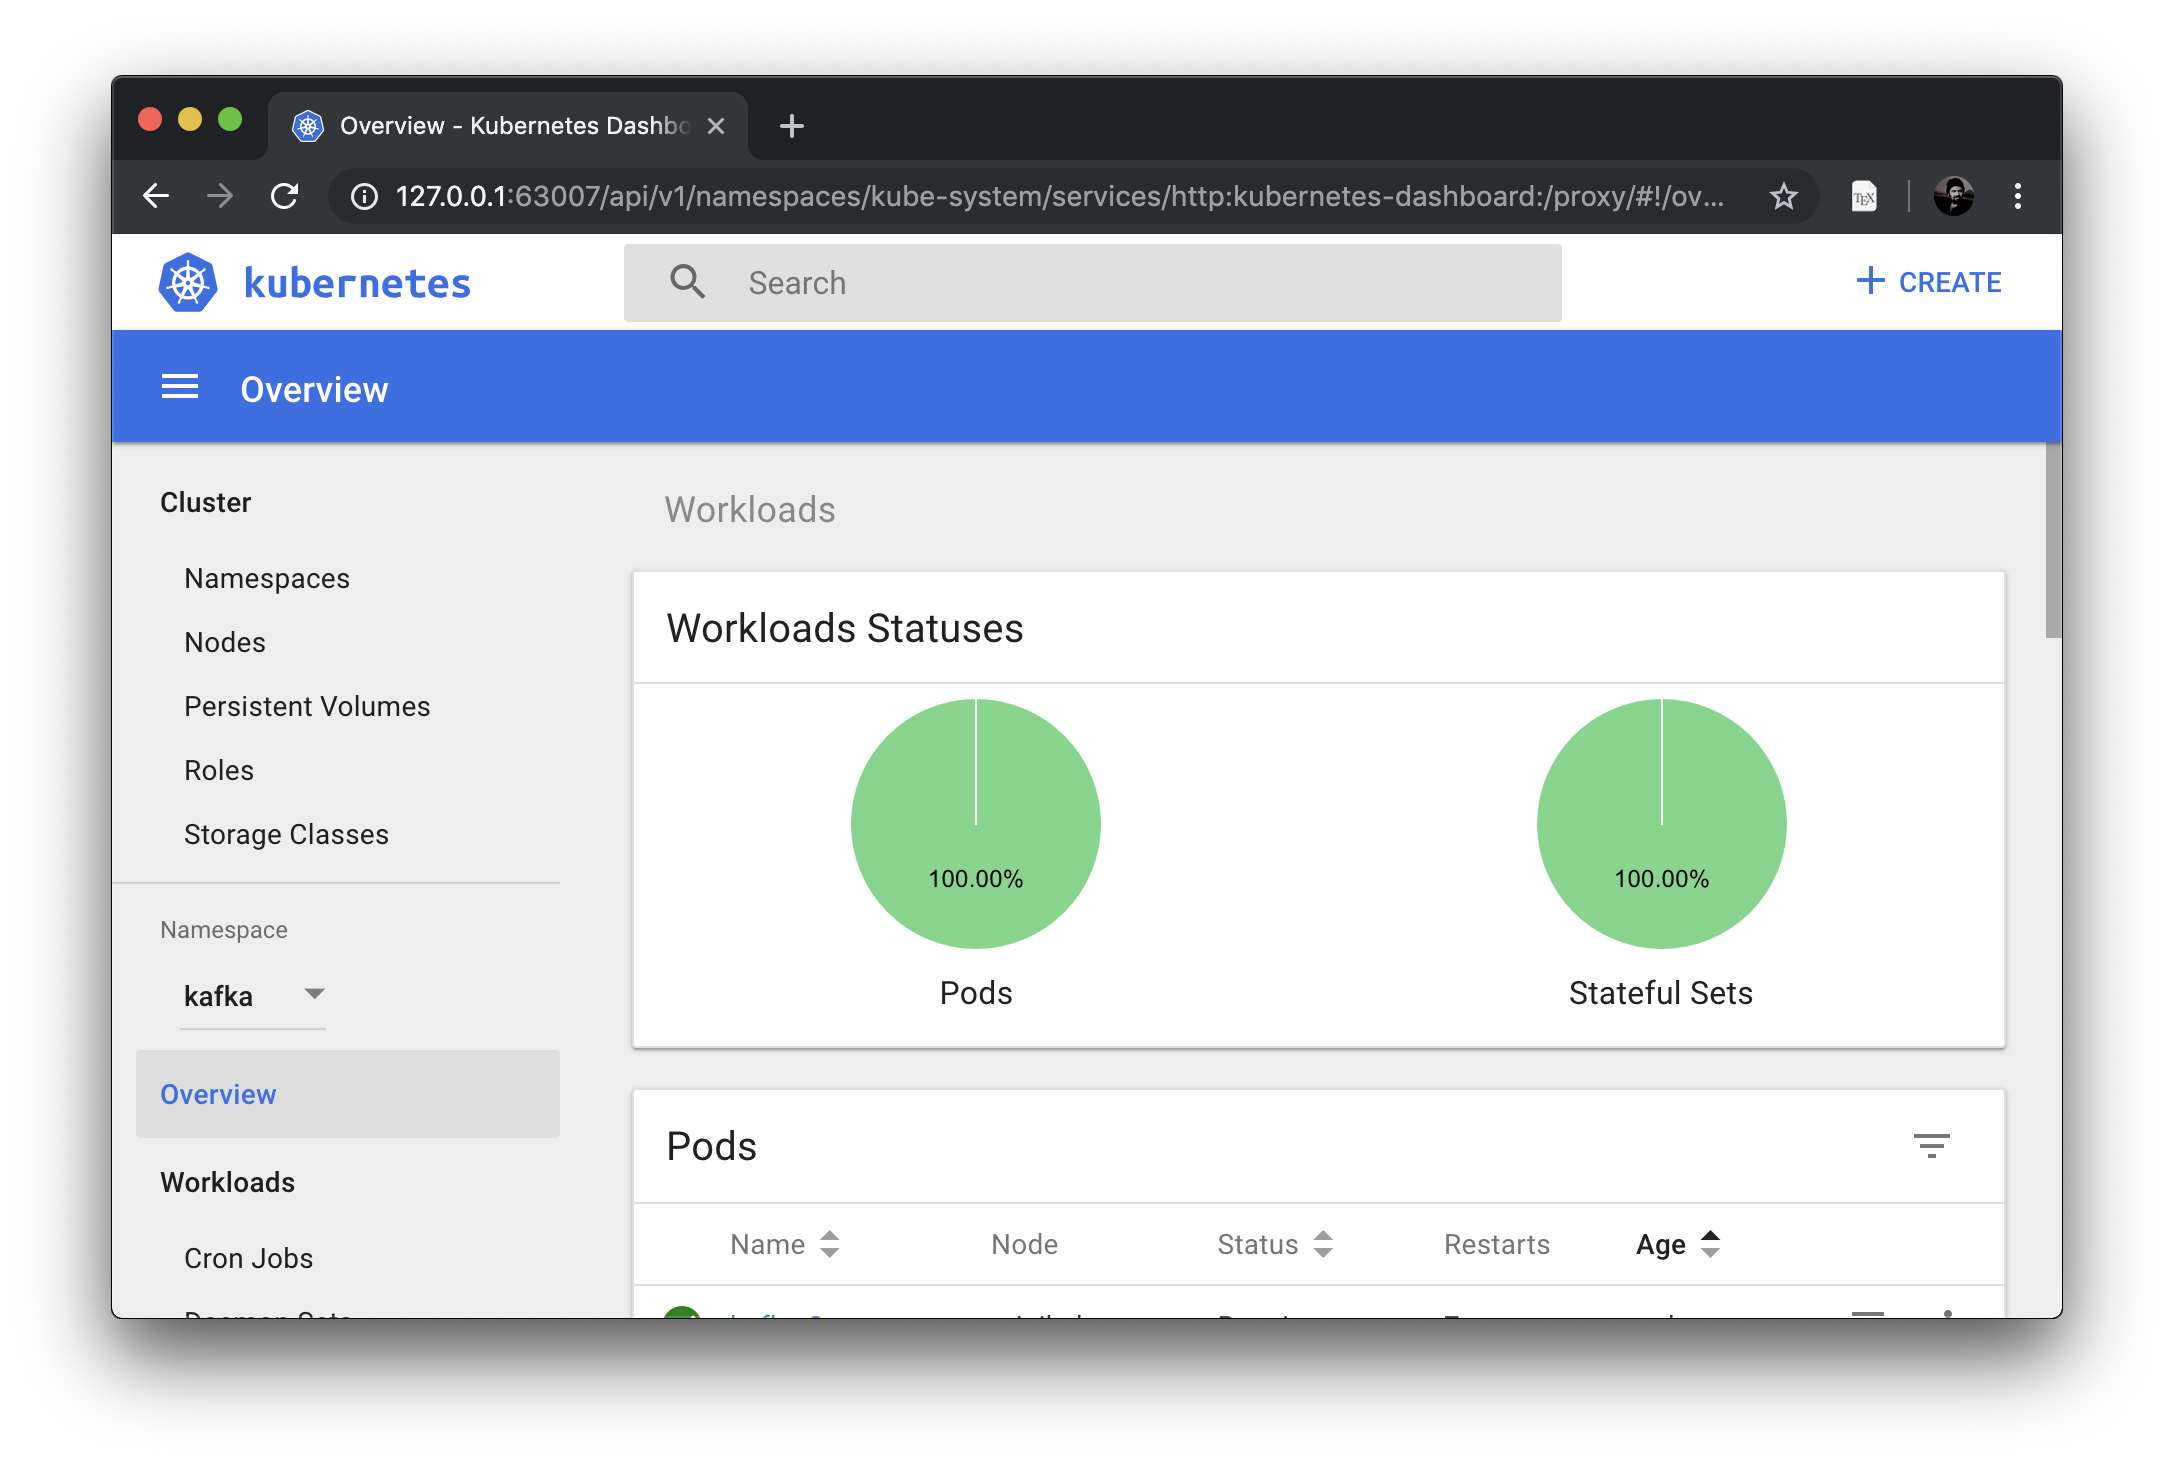
\includegraphics[width=\linewidth]{figures/appendixA/dashboard-kafka.png}
 	\caption{Minikube Dashboard status for the \texttt{kafka} namespace.}
 \end{figure}

 \item While cluster endpoints are typically exposed using Kubernetes Services, this approach presents some difficulties when exposing a Kafka bootstrap server, as the server presents clients with cluster-internal broker IP addresses which will not be resolvable by cluster-external clients. This issue can be circumvented by configuring a VPN into the cluster, using a solution such as \textit{Telepresence}. Install Telepresence by following the instructions at https://www.telepresence.io/.
 
 \item Start a VPN from your host OS to the Kubernetes cluster by executing the following command. As a prerequisite step, determine the cluster-inter Kafka broker IP address via the Minikube dashboard,
 
 \begin{lstlisting}[language=bash]
$ telepresence --run-shell --also-proxy broker.kafka --also-proxy zookeeper.kafka  
--also-proxy <kafka broker internal ip address>
\end{lstlisting}

 \begin{figure}[H]
	\centering  
	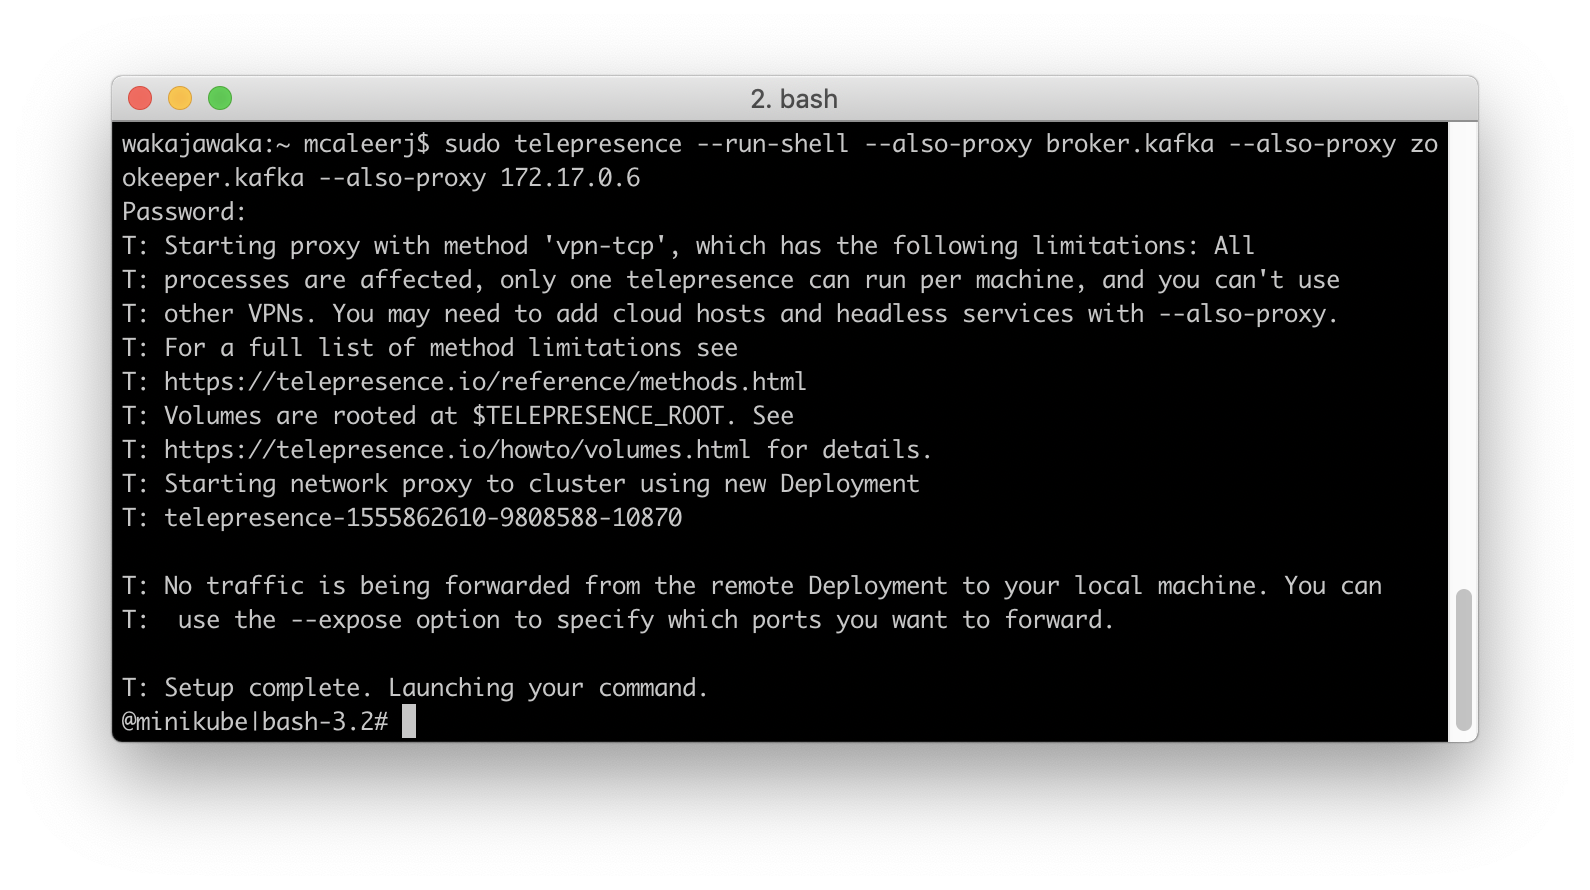
\includegraphics[width=\linewidth]{figures/appendixA/start-telepresence.png}
	\caption{Telepresence startup.}
\end{figure}

 \item To test cluster connectivity, start a Kafka console consumer, pointing it to the Kafka broker running within the Kubernetes cluster. As topic auto-creation is enabled, configure the tool to listen on an arbitrary topic such as \texttt{test-topic}:
 
  \begin{lstlisting}[language=bash]
 $ kafka-console-consumer --bootstrap-server bootstrap.kafka:9092 --topic test-topic
 \end{lstlisting}

 \item Next, send a message to the topic chosen in the previous step:
 
  \begin{lstlisting}[language=bash]
 $ kafka-console-producer --broker-list broker.kafka:9092 --topic test-topic
 \end{lstlisting}

 \begin{figure}[H]
	\centering  
	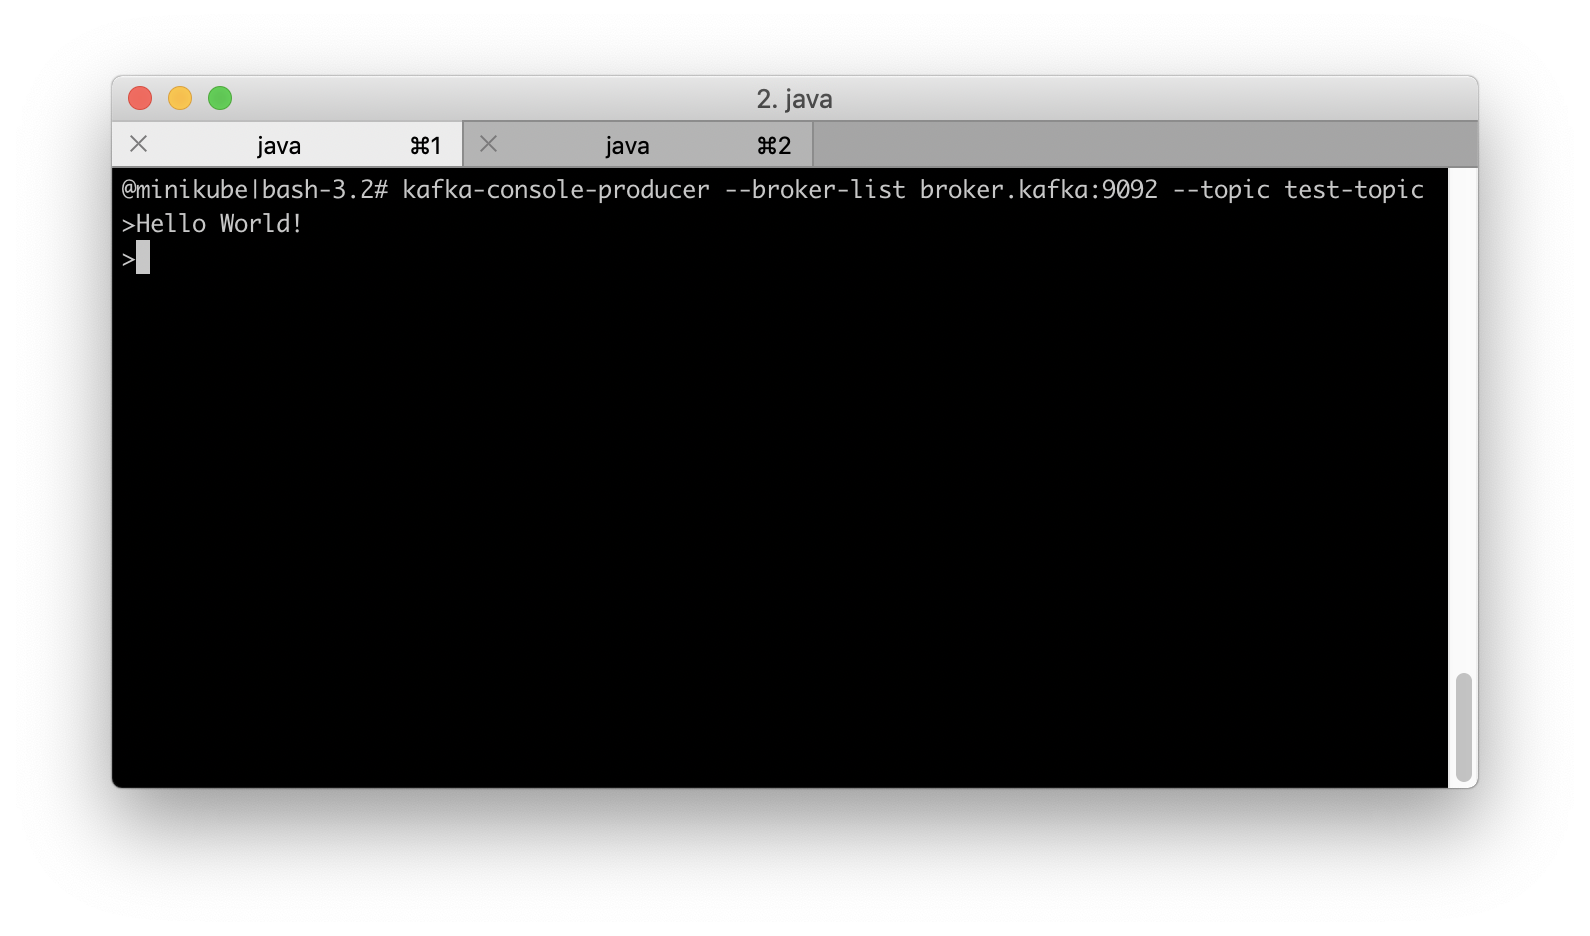
\includegraphics[width=\linewidth]{figures/appendixA/send-test-message.png}
	\caption{Sending a test message to topic \textit{test-topic}.}
\end{figure}


 \item The kafka consumer should now echo the text message. If so, the Zookeer/Kafka environment and Telepresence VPN are configured correctly.

\begin{figure}[H]
	\centering  
	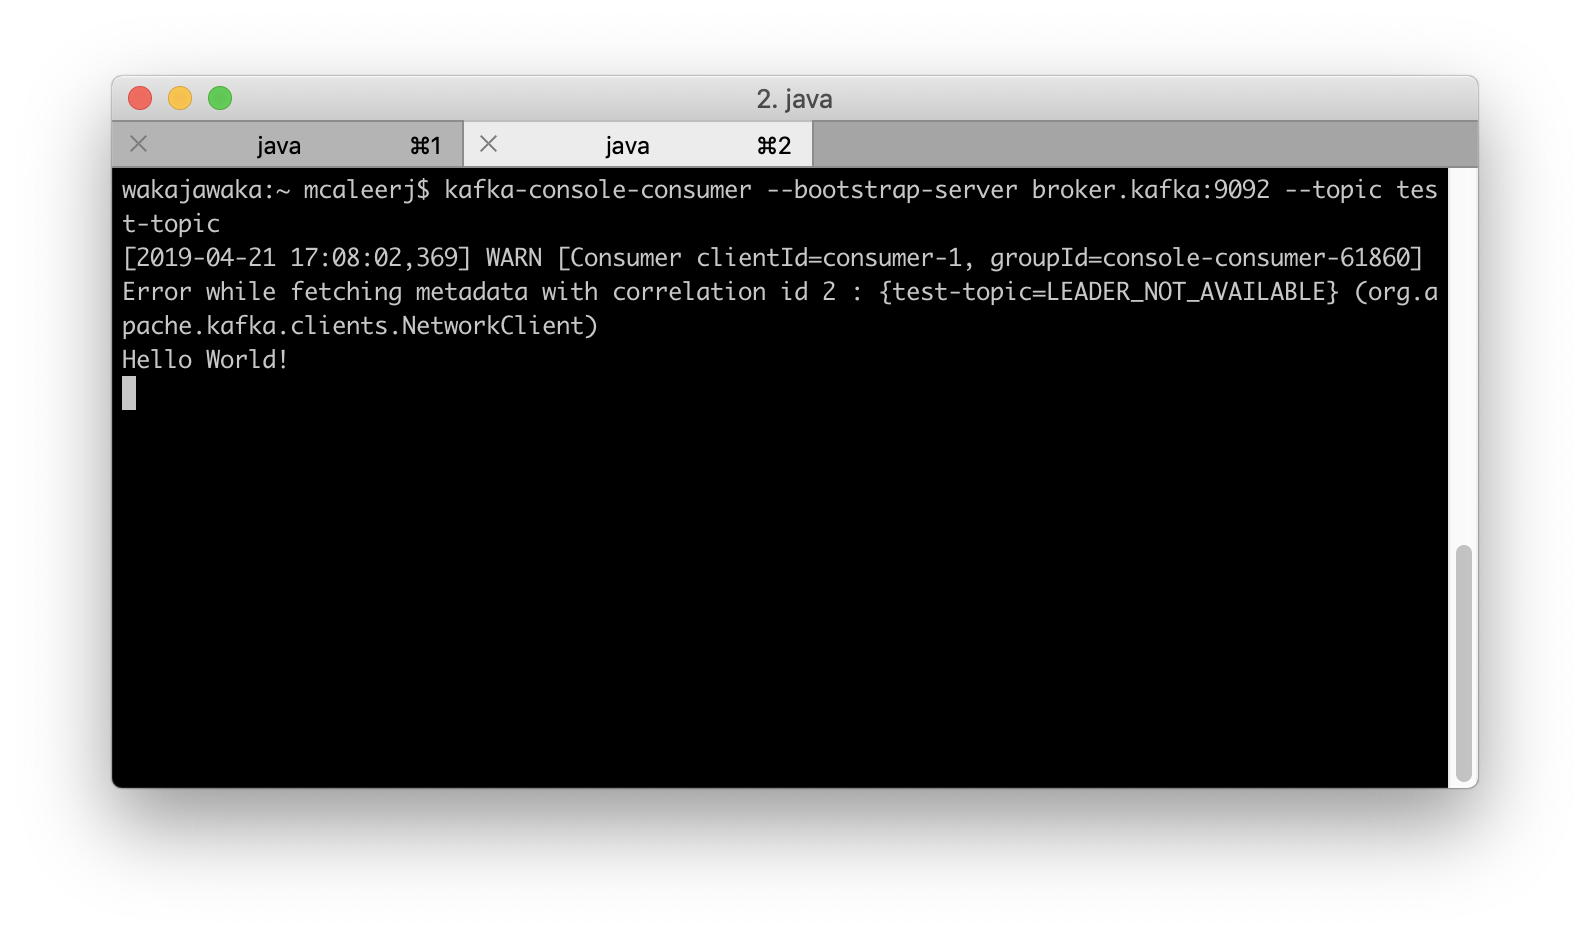
\includegraphics[width=\linewidth]{figures/appendixA/consume-test-message.png}
	\caption{Receiving a test message on topic \textit{test-topic}.}
\end{figure}


 \item Next, configure the test pipeline microservices. The various applications are bundled with the project implementation sources at https://github.com/schmigware/monitoring-app. Change directory to \texttt{/software/test-environment}. Execute the following commands to configure security roles and a new namespace,  \textbf{testbed}.

  \begin{lstlisting}[language=bash]
$ kubectl apply -f k8s/testbed-namespace.yml
$ kubectl apply -f k8s/serviceaccount.yml -n testbed
\end{lstlisting}

 \item Verify that the \texttt{testbed} namespace has been created correctly by issuing the following kubctl command:

\begin{lstlisting}[language=bash]
$ kubectl get namespaces
\end{lstlisting}

The output should list the expected namespace.

\begin{figure}[H]
	\centering  
	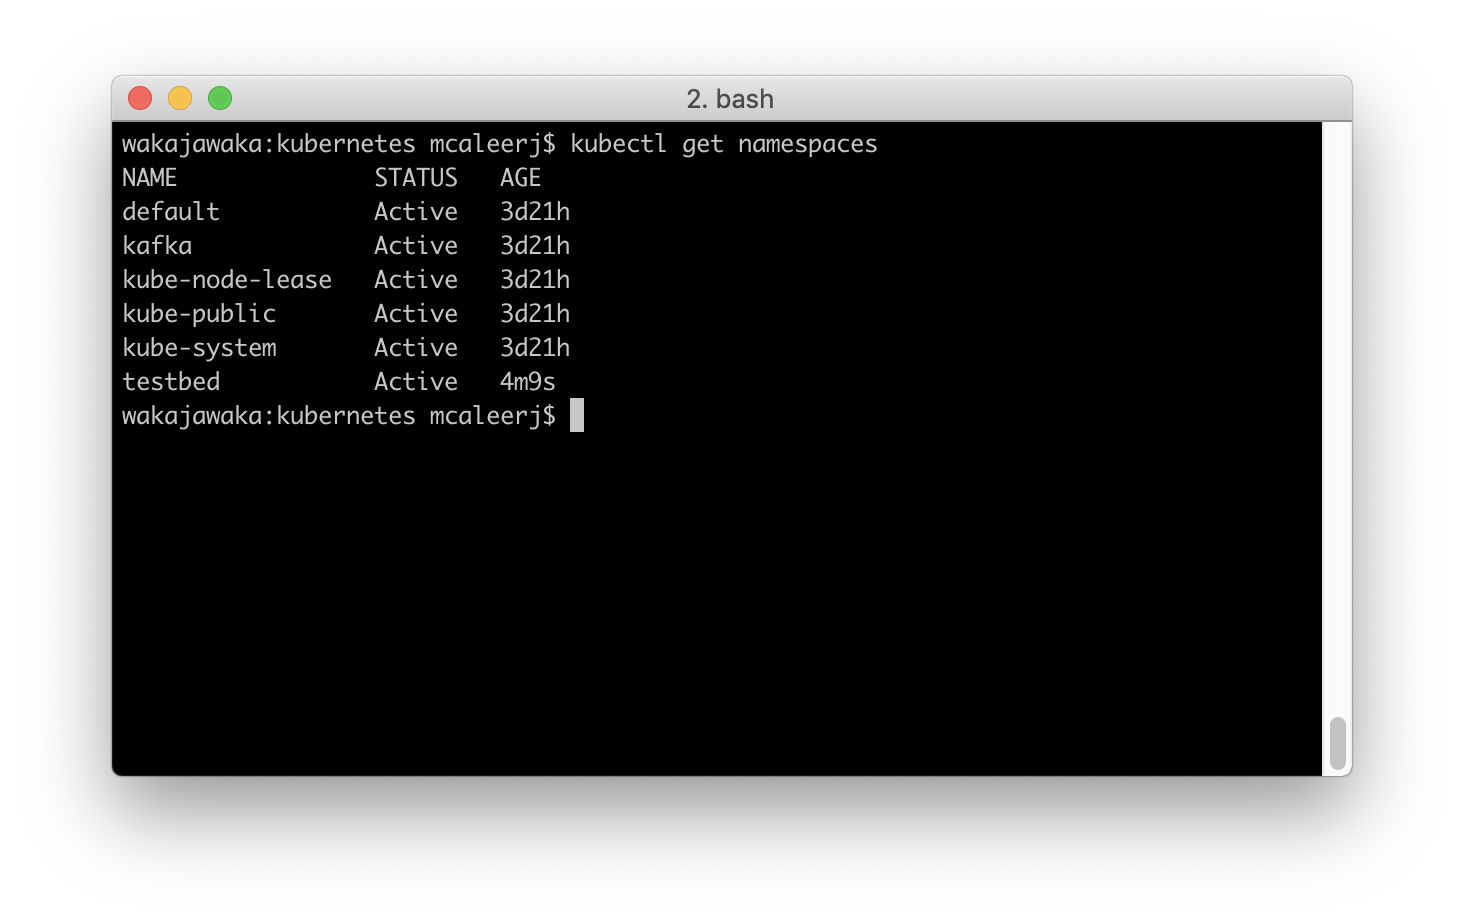
\includegraphics[width=\linewidth]{figures/appendixA/testbed-namespace.png}
	\caption{Verification of kafka namespace creation.}
\end{figure}

 \item Build the various microservice projects by issuing the following commands from the directory  \texttt{/software/test-environment}. The first shell command forces the Maven Docker build task to build microservice images using Minikube's Docker registry.
 
  \begin{lstlisting}[language=bash]
 $ eval $(minikube docker-env)  
 $ maven clean install
 \end{lstlisting}


\item Create Kubernetes deployments for the \textit{ingestion}, \textit{validation} and \textit{sink} test bed services by executing the following commands in order. 

\begin{lstlisting}[language=bash]

$ kubectl apply -f ingestion-service/application/k8s/configmap.yml
$ kubectl apply -f ingestion-service/application/k8s/deployment.yml

$ kubectl apply -f validation-service/application/k8s/configmap.yml
$ kubectl apply -f validation-service/application/k8s/deployment.yml

$ kubectl apply -f sink-service/application/k8s/configmap.yml
$ kubectl apply -f sink-service/application/k8s/deployment.yml
\end{lstlisting}

 \item Verify that the \texttt{testbed} namespace contains running microservice applications by issuing the following kubctl command, which lists all pods for the namespace in question:

\begin{lstlisting}[language=bash]
$ kubectl get pods -n testbed
\end{lstlisting}

The output should list three running pods:

\begin{figure}[H]
	\centering  
	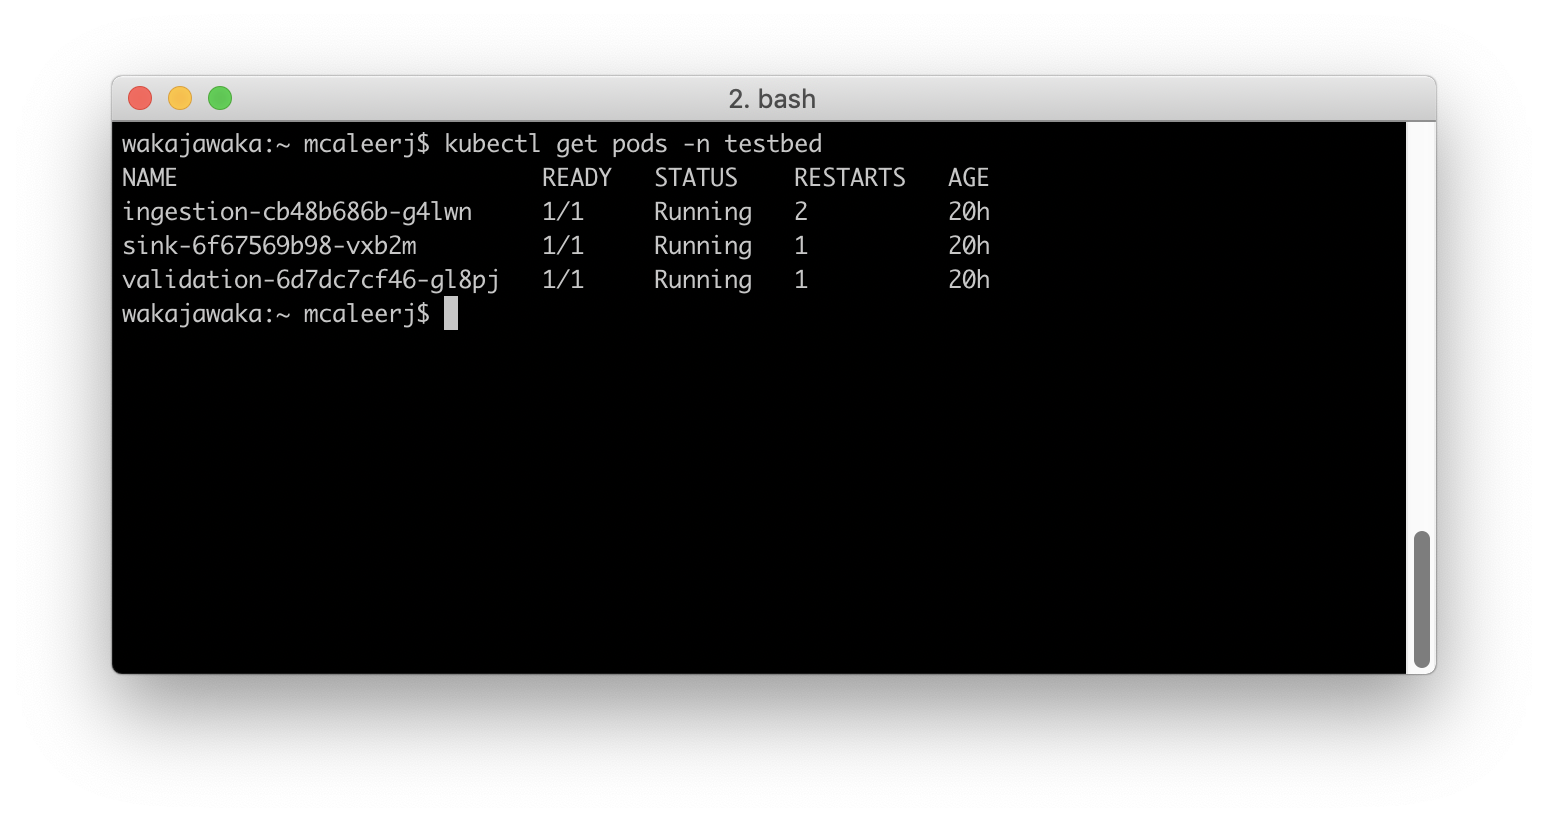
\includegraphics[width=\linewidth]{figures/appendixA/testbed-pods.png}
	\caption{Verification of test bed pod creation.}
\end{figure}

 \item Furthermore, the test bed pipeline microservices should be reflected in the Minikube dashboard:
 
 \begin{figure}[H]
 	\centering  
 	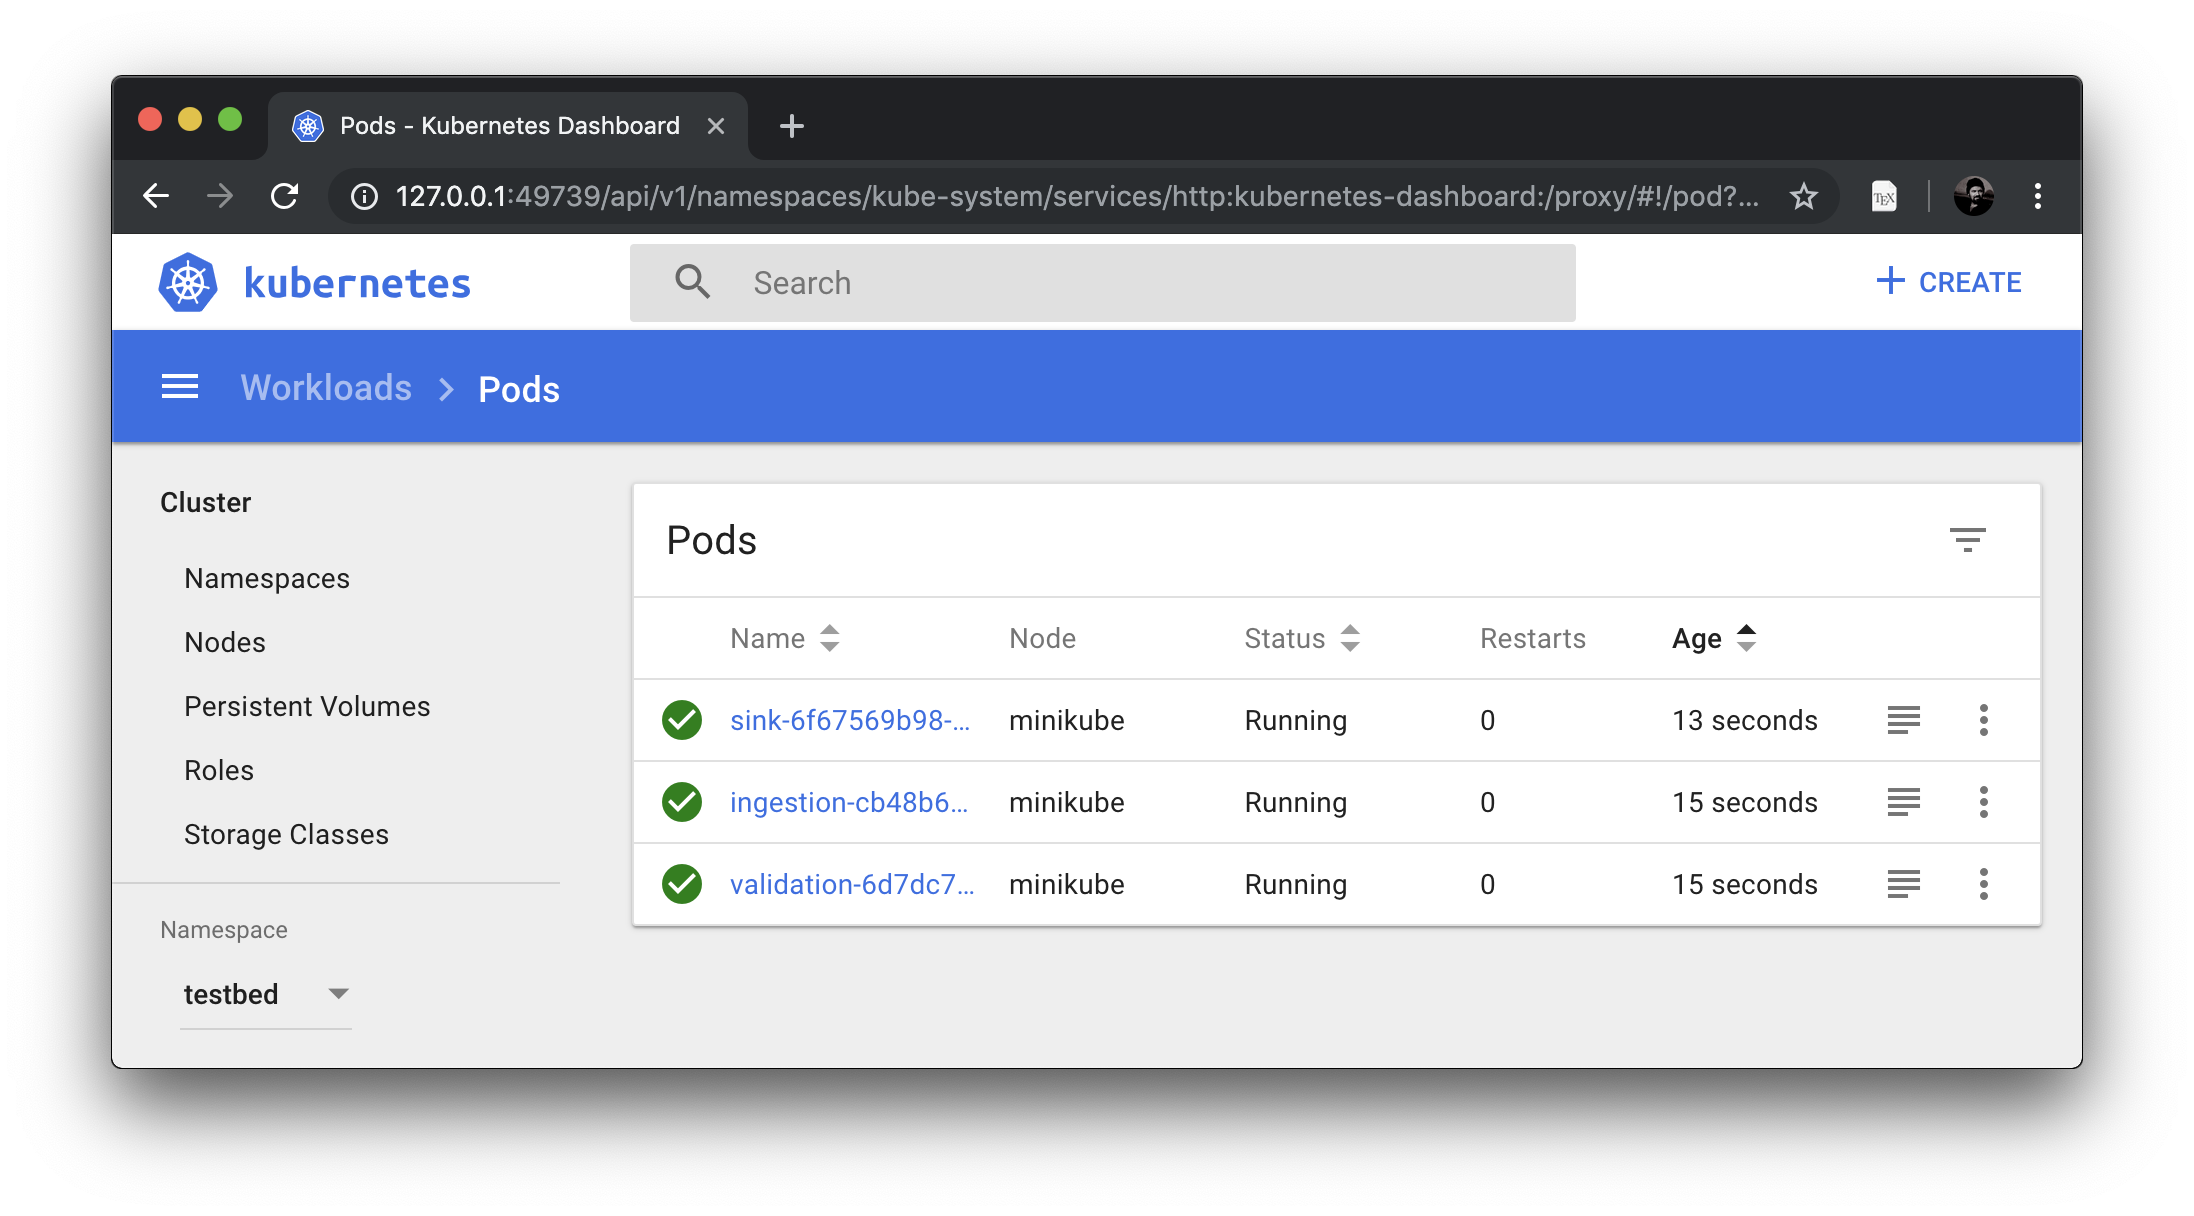
\includegraphics[width=\linewidth]{figures/appendixA/testbed-dashboard.png}
 	\caption{Test bed pod state at the Minikube dashboard.}
 \end{figure}


\end{enumerate}

\section{Verification}
 
 \begin{enumerate}

  \item Verify that messages can successfully traverse the test bed pipeline. A Python-based event generator provided with the project sources can be used to send a stream of test messages to the cluster's Kafka broker. To execute the message generator, change directory to \texttt{/software/message-generator} and execute the following command; the generator will send five messages per second to the broker on the topic \textbf{source}, the ingestion topic of the test pipeline:
  
  \begin{lstlisting}[language=bash]
  $ python generator.py -b bootstrap.kafka:9092 -t source -n5
  \end{lstlisting}

For each message sent, a single period character is echoed to the console:
 
  \begin{figure}[H]
 	\centering  
 	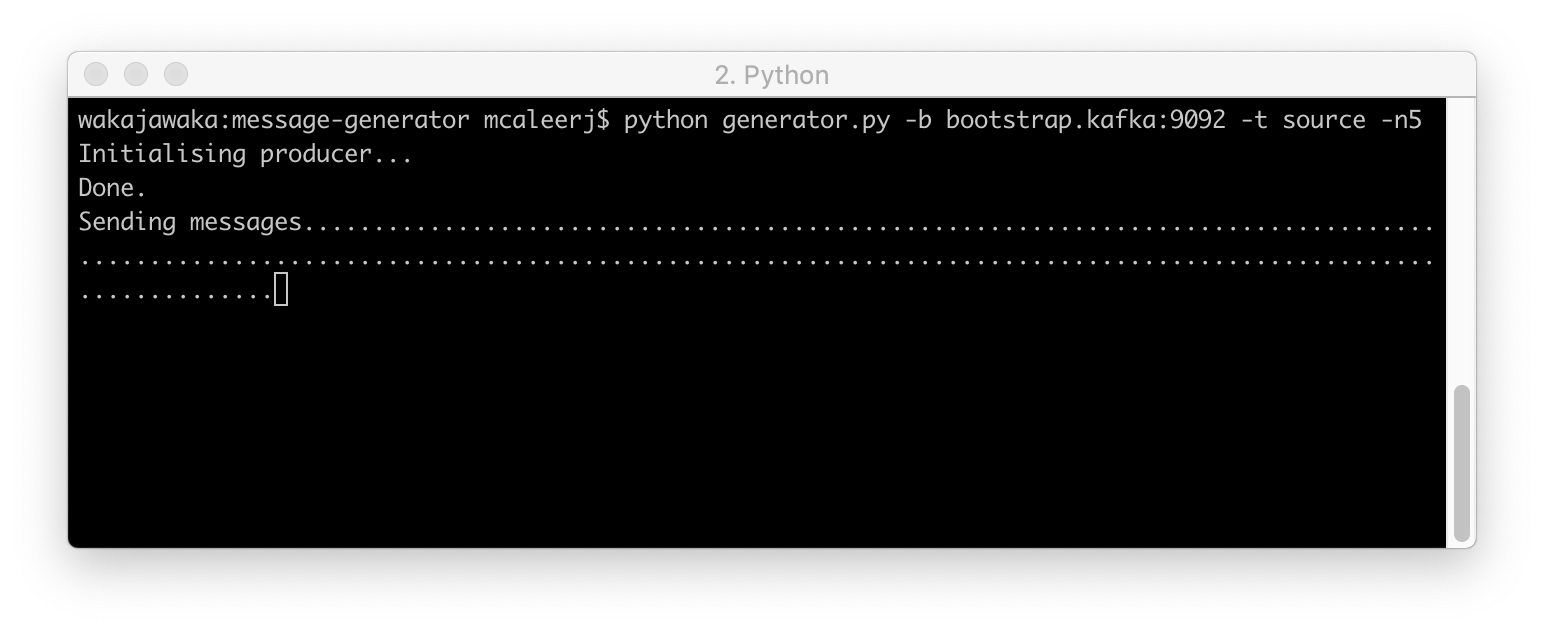
\includegraphics[width=\linewidth]{figures/appendixA/testbed-send-messages.png}
 	\caption{Sending test messages to the \textit{source} topic.}
 \end{figure}

Verify that messages are successfully traversing the pipeline by listening on the pipeline sink topic, \textit{processed}, using the following command:

  \begin{lstlisting}[language=bash]
$ kafka-console-consumer --bootstrap-server bootstrap.kafka:9092 --topic processed
\end{lstlisting}

 Test messages should be output as follows:
 
   \begin{figure}[H]
 	\centering  
 	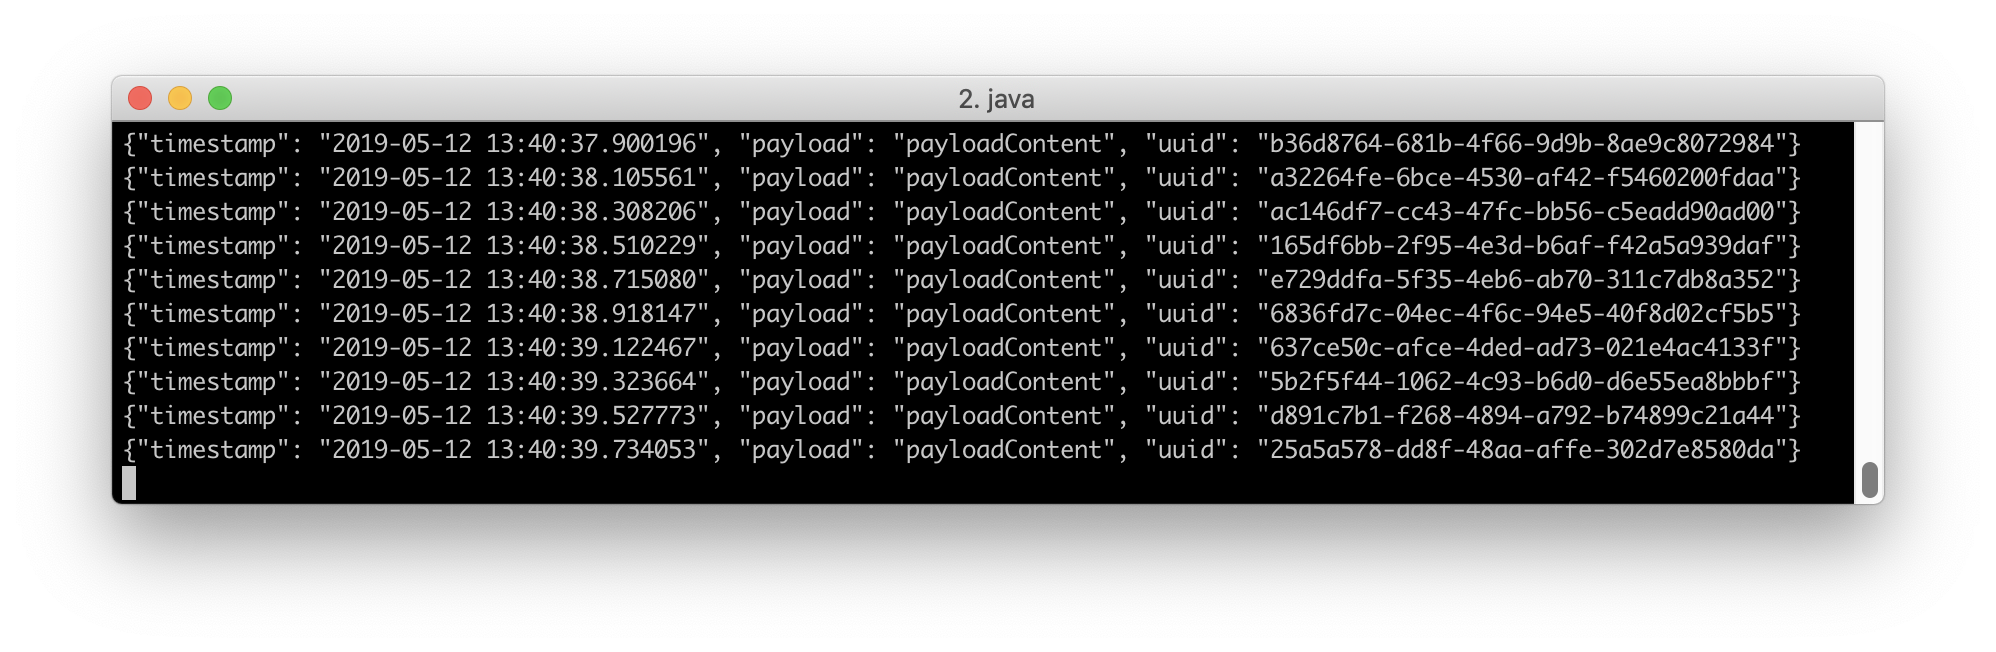
\includegraphics[width=\linewidth]{figures/appendixA/testbed-processed-messages.png}
 	\caption{Receiving test messages from the test pineline \texttt{processed} topic.}
 \end{figure}

The Kubernetes cluster is now successfully configured with Zooker and Kafka instances in namepace \texttt{kafka}. The test bed pipeline application is successfully processing messages in namespace \texttt{testbed}.
 
 
\end{enumerate}